\subsection{Benchmarking Goals}

The benchmarking methodology developed for this thesis is designed for the evaluation of the Ceph file system across diverse cluster configurations in order to assess its suitability for \ac{HPC} applications. To that end, we have deployed and evaluated two classes of Ceph clusters:

\begin{itemize}
    \item A simulated production environment (see~\cref{sec:production-deployment}), deployed with \texttt{cephadm}
    \item Custom in-memory deployments (see~\cref{sec:custom-deployment}), deployed with the Cuttlefish deployment tool developed for this thesis
\end{itemize}

In the production deployment, our benchmarking objectives are primarily qualitative and architectural evaluations. This deployment does not focus on peak performance measurements, as the constraints of the production deployment are controlled such that they are not expected to exceed Ceph's architectural capabilities. Instead, we have evaluated the orchestration process using \texttt{cephadm}, as well as analyzed potential deviations between theoretical performance models controlled by our performance throttling process and the observed behaviour of the cluster.

The in-memory deployment focuses primarily on quantitative stress testing in order to isolate Ceph's architectural performance limitations. These benchmarks are designed to evaluate Ceph's performance and scalability at various levels under high-load conditions, eliminating external compounding factors where possible. For instance, physical storage media such as hard drives and \acp{SSD} can have complex and potentially non-deterministic performance characteristics; using memory-backed \acp{OSD} eliminates disk performance as a source of potential performance bottlenecks. This methodology allows for an evaluation focused primarily on software overhead of the various layers of the Ceph file system, such as \ac{RADOS} and \ac{CephFS}, although other limiting factors such as memory and network bandwidth remain. 

\ac{IOR} and mdtest benchmark configurations were repeated 3 and 5 times respectively to account for random network jitter and other sources of variance. The higher repetition count for mdtest was chosen due to the higher observed variance in metadata operations compared to \ac{IOR}'s throughput measurements. Unless stated otherwise, the reported results are the mean across repetitions.

\subsubsection{Performance Testing}

Performance was evaluated through performance metrics obtained via two of its primary interfaces: the \ac{RADOS} object storage layer and \ac{CephFS}.

\ac{RADOS} performance benchmarks were used to establish a fundamental performance baseline, as it serves as the underlying storage method for all higher-level Ceph services, such as \ac{CephFS}, \ac{RBD}, and \ac{RGW}. As such, these measurements represent a theoretical \enquote{upper bound} of the cluster's throughput and \ac{I/O} capabilities at the lowest abstraction level.

The evaluation additionally includes \ac{CephFS} to assess performance in real-world deployments, such as the hosting of users' home directories or a high-performance scratch file system. In these scenarios, the overhead introduced by the implementation of a \ac{POSIX} compliant file system and its associated functionality is of particular concern. We have placed particular emphasis on metadata performance, as the \ac{MDS} daemons can represent a potential bottleneck, and common workloads such as the creation of Python virtual environments or compilation of software packages produce uniquely high-frequency bursts of small file \ac{I/O}.

A comparative analysis of \ac{RADOS} and \ac{CephFS} results with the same cluster configuration allows for the quantification of the overhead introduced specifically by the \ac{CephFS} file system abstraction layer.

\subsection{Benchmark Implementation}

\subsubsection{Modifications to \acs{IOR} and mdtest}
\label{sec:modifications-to-ior-mdtest}

During initial testing, bugs and limitations in \ac{CephFS} functionality within \ac{IOR} and mdtest were discovered and patched. The following components within the \ac{CephFS} backend were modified.

\begin{itemize}
    \item Addition of \texttt{mknod} and \texttt{rename} functionality, enabling the mdtest mknod folder creation and directory renaming tests
    \item Fix for the \texttt{CEPHFS\_StatFS} function to return correct index node utilization
\end{itemize}

These fixes enable full mdtest functionality on the \ac{CephFS} backend. Note
that the \ac{RADOS} backend, being an object store, does not provide a file
system structure to be tested. Therefore, \ac{RADOS} can only be tested with
\ac{IOR}.

In addition, the outputs provided by \ac{IOR} and mdtest are insufficient for
debugging, as they report only that operations have failed without exposing
additional details, such as error codes. This lack of information made issues
such as incorrect permissions or missing folders difficult to identify. The
programs were modified to emit detailed information on failure to address this
limitation. However, it does not affect the system's functionality and exists
purely as a debugging aid.

\subsubsection{Benchmarking Container Creation}

The Ceph image does not contain \ac{IOR} or mdtest on its own, and not all of
its dependencies were straightforward to install on Rocky Linux 8. This was
primarily due to the older software versions available in the package
repositories. Therefore, these were compiled from source on top of the existing
upstream Ceph container with a Dockerfile (see~\cref{appendix:ior-mdtest-dockerfile}).

The build script performs the following:

\begin{itemize}
    \item Installs the development headers and links \ac{IOR}/mdtest to the Ceph 
libraries, ensuring a version match with the containers on the server side.
    \item Installs Open \ac{MPI} to allow for communication between \ac{IOR} tasks.
    \item Enables the optional support for \acs{CephFS} and \acs{RADOS} within \ac{IOR}.
    \item Patches \ac{IOR}/mdtest to add the functionality specified in~\cref{sec:modifications-to-ior-mdtest}
\end{itemize}

Since the Docker build process outputs a Docker image, conversion into
Apptainer's native \ac{SIF} format is required. Apptainer provides functionality
to perform this conversion natively, however, there were some permission issues
experienced when building on top of the existing Ceph image. In order to fix
this, a simple shim script was created to run an Apptainer \texttt{-{}-fix-perms}
pass on the container image, which fixed issues experienced with running dnf in
the containers during debugging. The script is shown in~\cref{lst:sif-shim-fix-perms}.

\lstinputlisting[
    caption={\acs{SIF} Conversion Shim},
    label={lst:sif-shim-fix-perms},
    frame=single,
    breaklines=true
]{assets/cuttlefish/build_ior.sh}

The output container, \texttt{cf-bench-ior.sif}, is used specifically for
benchmarking. The unmodified Ceph container image is used for the daemons.

\subsubsection{Performance Scaling}

In order to evaluate and narrow down possible sources of performance bottlenecks, we will run performance tests using different combinations of clients and nodes. For instance, if a single node with 64 tasks performs worse than two nodes with 32 tasks each, it is possible that this is not a server-side bottleneck, but rather a client-side one, e.g., a compute or network bandwidth limitation.

To that end, a custom benchmarking script was developed which automates the running of various \ac{IOR} and mdtest configurations. The system shares some core components with the deployment system, such as the the Slurm interface, in order to determine the available nodes. The benchmarks are performed on the cluster based on the user's request and node allocation, and are saved to a database for further processing. The workflow is shown in~\cref{fig:cuttlefish-benchmark-flowchart}.

\begin{figure}[htbp]
    \centering
    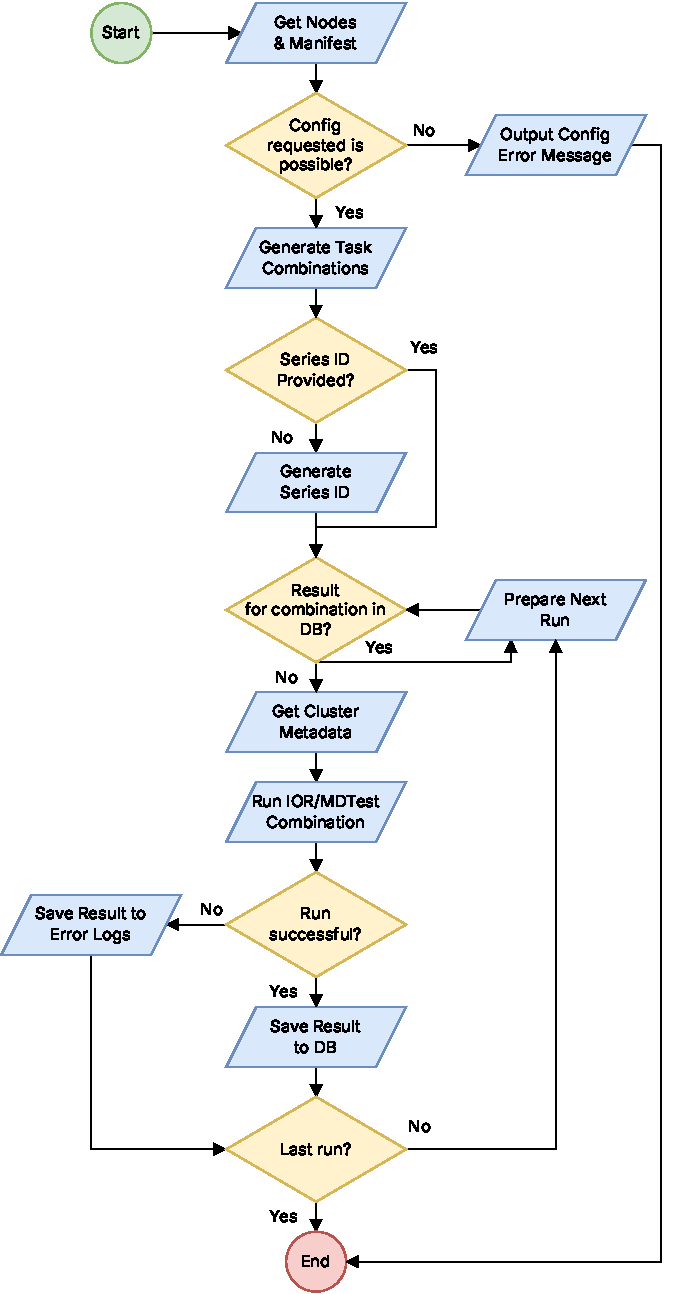
\includegraphics[width=0.7\linewidth]{assets/cuttlefish/benchmark_flowchart.pdf}
    \caption{Benchmarking Process Flowchart}
    \label{fig:cuttlefish-benchmark-flowchart}
\end{figure}

\subsubsection{Layout}

Two node types were tested: one with InfiniBand networking and one with
Omni-Path networking. All node types were running Rocky Linux 8.10 with the
kernel version 4.18.0-553.89.1.el8\_10.x86\_64.

The 16 InfiniBand test nodes were equipped with the hardware shown in
\cref{tbl:infiniband-system}.

\begin{table}[H]
\centering
\begin{tabular}{|ll|}
\hline
\textbf{Component} & \textbf{Specification} \\
\hline
CPU        & 2$\times$ AMD EPYC 7513 (32C/64T per CPU) \\
RAM        & 512 GB \\
Networking & 200 Gbps InfiniBand (NVIDIA ConnectX-6) \\
\hline
\end{tabular}
\caption{InfiniBand Test System Hardware}
\label{tbl:infiniband-system}
\end{table}

The Omni-Path nodes were equipped as shown in \cref{tbl:omnipath-system}.

\begin{table}[H]
\centering
\begin{tabular}{|ll|}
\hline
\textbf{Component} & \textbf{Specification} \\
\hline
CPU        & 2$\times$ Intel Xeon Platinum 8468 (48C/96T per CPU) \\
RAM        & 256 GB \\
Networking & 100 Gbps Omni-Path (Intel HFI100) \\
\hline
\end{tabular}
\caption{Omni-Path Test System Hardware}
\label{tbl:omnipath-system}
\end{table}

For all of the test systems, individual \acp{OSD} used the Memstore backend with
dynamic sizing, as described in~\cref{sec:ceph-autoconfig}. Due to the limited
number of available nodes, monitors are co-located with other daemon types on
the same node (e.g., \ac{MDS} daemons and \acp{OSD}).

\subsection{Data Collection}
\label{sec:data-collection}

By default, \ac{IOR} and mdtest emit human-readable data. They can also be
configured to output machine-readable data; \ac{IOR} can output \ac{JSON}
formatted data, while mdtest can output \ac{CSV} formatted data. However, some
challenges were faced when programmatically parsing the data:

\begin{itemize}
    \item Both \ac{IOR} and mdtest do not provide a formally specified data schema for their outputs, which complicates the inspection of output data.
    \item Units for bandwidth metrics in \ac{IOR} are expressed interchangeably in kilobytes and megabytes.
    \item The use of case is inconsistent throughout the output. For example, individual tests have the key \texttt{TestID}, while the test parameters have the key \texttt{testID}.
    \item Summary statistics are not directly associated with performed tests, complicating the attribution of summaries to test results for analysis.
\end{itemize}

In order to allow for easier result aggregation as well as more efficient storage of test results, data pass through a three-step process consisting of parsing, normalization, and database storage.

\subsubsection{\acs{IOR} Result Parsing}

Pydantic is used to parse \ac{IOR} results from the result \ac{JSON} data directly through conversion of field names and normalization of units. A snippet is shown in~\cref{lst:ior-result-pydantic} for a single \ac{IOR} result. Additional functions and Pydantic models are used for unit conversion and to cover the rest of the \ac{IOR} output, although they are not shown here.

\lstinputlisting[
    caption={[\acs{IOR} Result Pydantic Model]Pydantic model for the results gathered from a single \acs{IOR} repetition. Units are normalized to bytes per second, types are strongly defined, and validation of these types are performed by Pydantic. Keys use consistent snake-case throughout all models, regardless of the input case of the \acs{IOR}/mdtest data.},
    label={lst:ior-result-pydantic},
    frame=single,
    breaklines=true,
    language=python
]{assets/ior/ior_result.py}


\subsubsection{MDTest Result Parsing}

The \ac{CSV}-formatted results from mdtest cannot be parsed directly by Pydantic. Therefore, the fields are first read by the Python \texttt{csv} module, and the corresponding Pydantic models are generated using a conversion function. As opposed to \ac{IOR}, mdtest does not provide details such as the number of nodes or tasks, and therefore these must be provided separately in order for these metrics to be tracked. As the benchmarking script controls the instantiation of the mdtest runs and has the required information, this is passed through to the mdtest result parser, part of which is shown in~\cref{lst:mdtest-parser}.

\lstinputlisting[
    caption={[mdtest Result Parsing Logic]Snippet of code used to convert raw \acs{CSV} data output by mdtest into Pydantic mdtest models.},
    label={lst:mdtest-parser},
    frame=single,
    breaklines=true,
    language=python
]{assets/ior/mdtest_parser.py}

\subsubsection{Data Storage}

Once raw data have been converted into the exchange format, i.e., the Pydantic
models, they are normalized before being saved to a SQLite database. This
provides more flexibility when aggregating results due to the fact that all data
are saved in a single location and do not have to, for example, be manually read
from multiple output files. This is also more efficient for large numbers of
results, as the processing of text data (i.e., \ac{JSON}/\ac{CSV} outputs) must
only be performed once during the conversion step before being stored in an
efficient database-native format.

\begin{figure}[H]
    \centering
    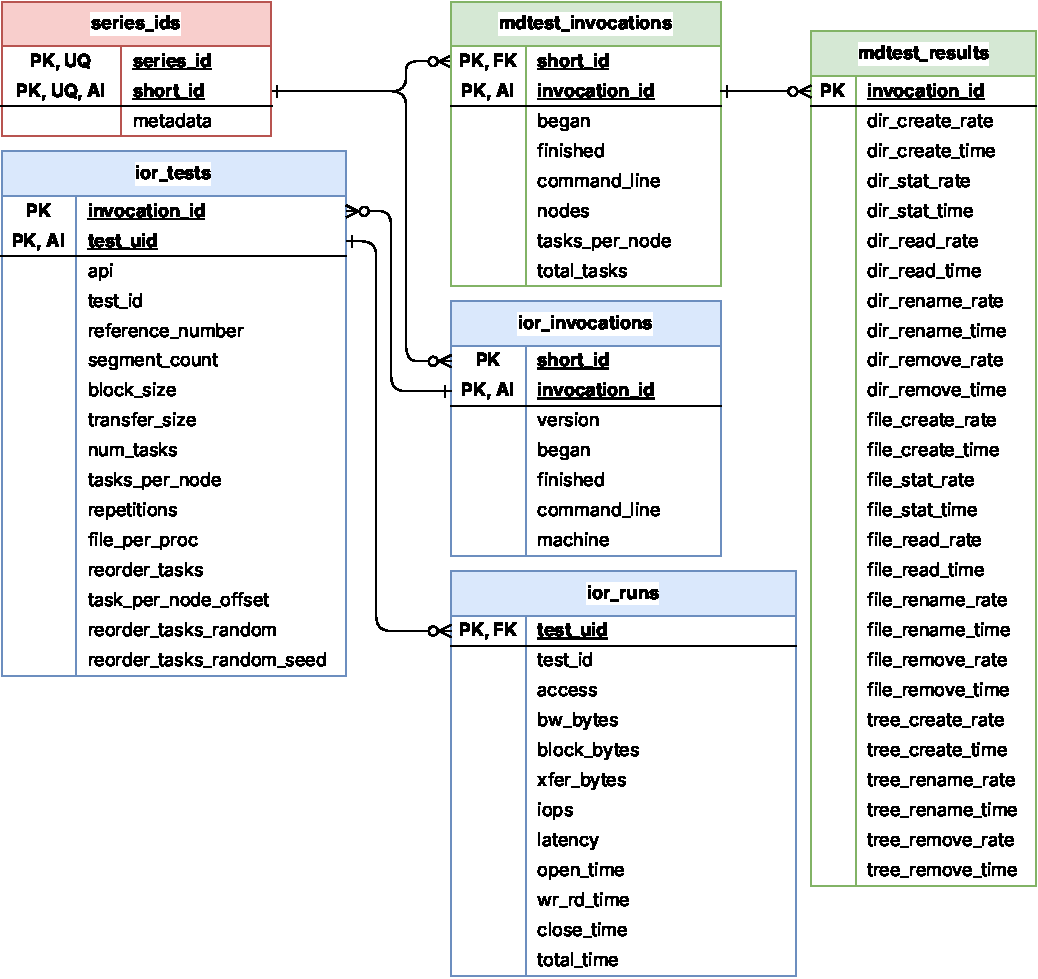
\includegraphics[width=\linewidth]{assets/cuttlefish/result-db-erd.pdf}
    \caption[Result Database ER Diagram]{\ac{ER} diagram of the result database, parsed from \acs{JSON} and \acs{CSV} data produced by \ac{IOR} and mdtest.}
    \label{fig:result-db-erd}
\end{figure}

\pagebreak

% In order to evaluate Ceph's performance characteristics, a benchmarking script
% runs multiple iterations of the \ac{IOR} benchmark with varied benchmark settings,
% numbers of client nodes and processes per node. To mimic a real-world
% deployment, the Ceph daemons and client nodes will be placed on separate
% machines. 

